%!TEX root = ../paper.tex

\tikzstyle{vertex} = [circle,draw,scale=.7,node distance=40pt]
\tikzstyle{vertex2} = [rectangle,draw,scale=1,node distance=100pt]
\tikzstyle{edge} = [->,line width=.2pt]
\tikzstyle{label} = [midway,below]
\def\offset{.1}

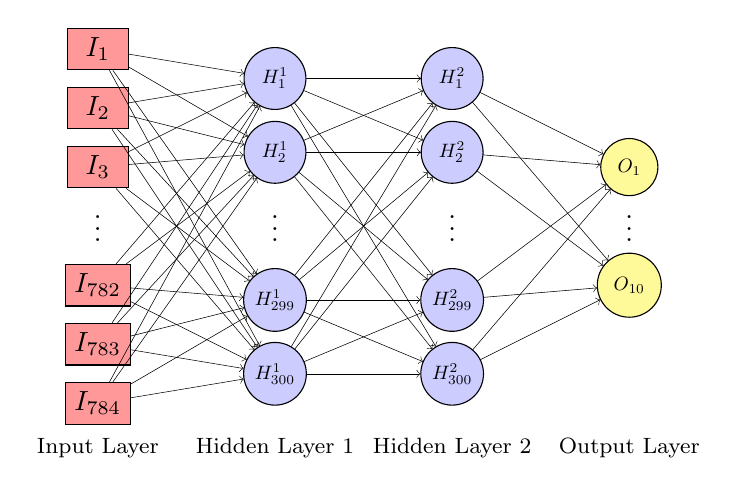
\begin{tikzpicture}[scale=.75]

% vertices
\node[vertex2,fill=red!40] (i1) at (-6,3) {$\ I_1\ $};
\node[vertex2,fill=red!40] (i2) at (-6,2) {$\ I_2\ $};
\node[vertex2,fill=red!40] (i3) at (-6,1) {$\ I_3\ $};
\node (idots) at (-6,.1) {$\vdots$};
\node[vertex2,fill=red!40] (i4) at (-6,-1) {$I_{782}$};
\node[vertex2,fill=red!40] (i5) at (-6,-2) {$I_{783}$};
\node[vertex2,fill=red!40] (i6) at (-6,-3) {$I_{784}$};

\node[vertex,fill=blue!20] (m1) at (-3,2.5) {$\ H_1^1\ $};
\node[vertex,fill=blue!20] (m2) at (-3,1.25) {$\ H_2^1\ $};
\node (mdots) at (-3,.1) {$\vdots$};
\node[vertex,fill=blue!20] (m3) at (-3,-1.25) {$H_{299}^1$};
\node[vertex,fill=blue!20] (m4) at (-3,-2.5) {$H_{300}^1$};

\node[vertex,fill=blue!20] (n1) at (0,2.5) {$\ H_1^2\ $};
\node[vertex,fill=blue!20] (n2) at (0,1.25) {$\ H_2^2\ $};
\node (ndots) at (0,.1) {$\vdots$};
\node[vertex,fill=blue!20] (n3) at (0,-1.25) {$H_{299}^2$};
\node[vertex,fill=blue!20] (n4) at (0,-2.5) {$H_{300}^2$};

\node[vertex,fill=yellow!40] (o1) at (3,1) {$\ O_{1}\ $};
\node (odots) at (3,.1) {$\vdots$};
\node[vertex,fill=yellow!40] (o2) at (3,-1) {$\ O_{10}\ $};

% edges
\foreach \i in {1,...,6} {
    \foreach \m in {1,...,4} {
        \draw[edge] (i\i) -- (m\m);
    }
}
\foreach \m in {1,...,4} {
    \foreach \n in {1,...,4} {
        \draw[edge] (m\m) -- (n\n);
    }
}

\foreach \n in {1,...,4} {
    \foreach \o in {1,...,2} {
        \draw[edge] (n\n) -- (o\o);
    }
}

% layer labels
\node at (-6,-3.75) {\footnotesize Input Layer};
\node at (-3,-3.75) {\footnotesize Hidden Layer 1};
\node at (0,-3.75) {\footnotesize Hidden Layer 2};
\node at (3,-3.75) {\footnotesize Output Layer};
    

\end{tikzpicture}